% Standalone theory note. General statistical laws are primary; Gaussian
% families are optional computational realizations only.
\documentclass[11pt,letterpaper]{article}

\usepackage[margin=0.92in]{geometry}
\usepackage{amsmath,amssymb,amsthm,mathtools}
\usepackage{bm}
\usepackage{booktabs}
\usepackage{xcolor}
\usepackage{microtype}
\usepackage{tikz}
\usetikzlibrary{arrows.meta,positioning,calc,fit,backgrounds}
\usepackage[hidelinks]{hyperref}

\newcommand{\KL}{D_{\mathrm{KL}}}
\newcommand{\E}{\mathbb E}
\newcommand{\cF}{\mathcal F}
\newcommand{\cG}{\mathcal G}
\newcommand{\cC}{\mathcal C}
\newcommand{\push}{_{\#}}
\newcommand{\Bern}{\operatorname{Bern}}
\newcommand{\logit}{\operatorname{logit}}
\newcommand{\sigmoid}{\operatorname{sigmoid}}
\newcommand{\grad}{\operatorname{grad}}

\definecolor{agentblue}{RGB}{46,105,157}
\definecolor{edgered}{RGB}{177,72,57}
\definecolor{parentgreen}{RGB}{63,128,90}
\definecolor{fieldorange}{RGB}{195,123,45}
\definecolor{softgray}{RGB}{238,241,244}

\newtheorem{definition}{Definition}
\newtheorem{proposition}{Proposition}
\newtheorem{remark}{Remark}

\title{Annealed Gauge-Covariant Belief Networks and a\\
Grand-Canonical Theory of Meta-Agent Formation}
\author{Gauge-Theoretic Multi-Agent Variational Free-Energy Program}
\date{August 16, 2026}

\begin{document}
\maketitle

\begin{abstract}
Variational free energy has the information-theoretic form of an expected energy minus an entropy.  In a multi-agent extension, gauge-transported relative entropies supply interaction energies while entropy-regularized attention supplies a Gibbs distribution over possible information sources.  Because beliefs, transports, and attention weights can evolve together, the existing construction is naturally an annealed network: node states and effective bonds coevolve.  This note first develops that network without assuming that any cluster is already a meta-agent.  It then introduces a separate grand-canonical topology in which the number of active edges can fluctuate, followed by a grand-canonical membership law for constructing pointwise meta-agents and a recursive network of meta-agents across scales.  A row-normalized attention weight is an occupation probability conditioned on choosing a source, not a chemical potential.  A genuine grand-potential term appears when edge or membership number itself fluctuates.  Binary occupations yield a lattice-gas form, with an explicit chemical potential controlling network density or meta-agent size and a transported divergence acting as gauge-invariant bond frustration.  A mean-field reduction exhibits a calculable coherence instability, while full joint gradient flow gives a Lyapunov law under fixed controls.  Sustained nonequilibrium, autonomous agency, and identification with physical thermodynamics require additional dynamical and operational assumptions.  The construction is stated for general normalized probability laws; multivariate Gaussian families are optional numerical realizations rather than foundations of the theory.
\end{abstract}

\section{Claim status and physical scope}

Three levels of assertion must remain separate.  The Helmholtz decomposition, canonical attention law, grand-occupation minimizer, gauge covariance, and gradient-flow balance are mathematical consequences of the stated functionals and assumptions.  The grand-canonical edge and membership functionals are proposed additions to the present theory.  Their identification with physical heat, work, particles, or chemical reservoirs is open and requires a separate operational bridge.

Variational free energy is dimensionless when logarithms are measured in nats.  Multiplication by $k_{\mathrm B}T_{\mathrm{phys}}$ gives energy units only after a physical Gibbs identification has been justified.  Friston described variational free energy as information-theoretic while emphasizing that its energy-minus-entropy form connects it to statistical thermodynamics~\cite{Friston2010}.  The use of ensemble mathematics here follows the inferential statistical mechanics of Jaynes~\cite{Jaynes1957}.  The mathematics of a Gibbs ensemble can therefore be exact even when the physical thermodynamic interpretation remains a modeling hypothesis.

The central conclusion can be stated immediately.  The present entropy-retaining attention row is a finite canonical Gibbs ensemble.  Jointly changing the beliefs and attention weights makes it an annealed canonical ensemble.  It does not become grand-canonical until the total number of edges or members is allowed to fluctuate under a conjugate chemical potential.

\section{Helmholtz structure of the multi-agent functional}

Let $q_i$ be a normalized belief law, $p_i$ its prior, and $L_i(o_i\mid z_i,c_i)$ its likelihood.  Let $\Omega_{ij}$ transport the belief law of agent $j$ into the local frame of agent $i$, and define
\begin{equation}
 r_{ij}:=(\Omega_{ij})\push q_j,
 \qquad
 D_{ij}:=\KL(q_i\Vert r_{ij}).
 \label{eq:transported-divergence}
\end{equation}
The canonical belief-channel functional for receiver $i$ is
\begin{equation}
 \boxed{
 \cF_i
 =\alpha_i\KL(q_i\Vert p_i)
 -\E_{q_i}\log L_i(o_i\mid z_i,c_i)
 +\sum_j\beta_{ij}D_{ij}
 +\tau_i\KL(\beta_i\Vert\pi_i)
 +R_i(\alpha_i).}
 \label{eq:canonical-agent-vfe}
\end{equation}
The row satisfies $\beta_{ij}\geq0$ and $\sum_j\beta_{ij}=1$.  The reference row is $\pi_i$ and $\tau_i>0$ is its attention temperature.  The symbol $\alpha_i$ without a channel superscript is the self-prior precision.  If it is optimized, its regularizer is not optional; the established adaptive form is $R_i(\alpha_i)=b_0\alpha_i-c_0\log\alpha_i$.  The separate $\alpha_i^q$ is an external receiver occupancy, giving the marked edge-event law $\eta_{ij}^q=\alpha_i^q\beta_{ij}$.

Expanding the relative entropies gives
\begin{align}
 \cF_i
 &=\E_{q_i}\left[
 -\alpha_i\log p_i
 -\log L_i
 -\sum_j\beta_{ij}\log r_{ij}
 \right]
 -\left(\alpha_i+\sum_j\beta_{ij}\right)H[q_i]
 \nonumber\\
 &\quad+\tau_i\KL(\beta_i\Vert\pi_i)+R_i(\alpha_i).
 \label{eq:helmholtz-expansion}
\end{align}
This is exactly an effective energy minus an entropy.  The prior, likelihood, and transported peer laws define the energy landscape.  The entropy of $q_i$ appears with coefficient $\alpha_i+1$ on a normalized attention row.  Changing individual $\beta_{ij}$ therefore changes the composition of the interaction field rather than the row's total entropy coefficient.

For fixed $\beta_i$ and normalizable factors, the stationary law is the logarithmic pool
\begin{equation}
 q_i^*(z)
 \propto
 \left[
 p_i(z)^{\alpha_i}
 L_i(o_i\mid z,c_i)
 \prod_j r_{ij}(z)^{\beta_{ij}}
 \right]^{1/(\alpha_i+1)}.
 \label{eq:belief-geometric-pool}
\end{equation}
The peer terms thus behave as genuine interaction fields.  This statement uses only normalized laws and finite relative entropies; it does not require Gaussian beliefs.

\section{Stage I: an adaptive network of agents without meta-agents}

The starting population contains only fine agents.  Every node carries its own belief, prior, likelihood, generative-model law, and gauge frame.  The graph supplies possible communication channels, but there is no parent variable, no coarse channel, and no claim that a coherent cluster is already an agent.  This ordering prevents the conclusion from being inserted into the premises.

The support or mask says which directed sources are admissible.  The attention row gives a conditional probability over those sources.  The beliefs determine transported mismatch energies, and the row free energy determines how a receiver allocates attention.  If the support stays fixed while $q$, $\Omega$, and $\beta$ evolve, interaction strength is adaptive but topology is fixed.  The network becomes topologically adaptive only after a separate edge-occupation variable is introduced.

\subsection{The correct row free energy}

For fixed beliefs and transports, the row scalar is
\begin{equation}
 \boxed{
 \cF_i^{\mathrm{row}}(\beta_i)
 =\sum_j\beta_{ij}D_{ij}
 +\tau_i\KL(\beta_i\Vert\pi_i),
 \qquad \sum_j\beta_{ij}=1.}
 \label{eq:row-free-energy}
\end{equation}
The entropy term cannot be omitted when $\beta_i$ is optimized.  The entropy-suppressed product $\sum_j\beta_{ij}D_{ij}$ is a different objective and has a different derivative after the row responds to the beliefs.

\begin{proposition}[Canonical attention ensemble]
If $\tau_i>0$ and $\pi_{ij}>0$ on the admitted source set, Eq.~\eqref{eq:row-free-energy} has the unique minimizer
\begin{equation}
 \beta_{ij}^*
 =\frac{\pi_{ij}\exp(-D_{ij}/\tau_i)}{Z_i},
 \qquad
 Z_i=\sum_k\pi_{ik}\exp(-D_{ik}/\tau_i),
 \label{eq:gibbs-attention}
\end{equation}
with reduced value and envelope differential
\begin{equation}
 \cF_{i,\mathrm{red}}^{\mathrm{row}}
 =-\tau_i\log Z_i,
 \qquad
 d\cF_{i,\mathrm{red}}^{\mathrm{row}}
 =\sum_j\beta_{ij}^*dD_{ij}.
 \label{eq:row-envelope}
\end{equation}
\end{proposition}

\begin{proof}
The row objective is strictly convex on the probability simplex.  A multiplier for normalization gives
\begin{equation}
 D_{ij}+\tau_i\left(1+\log\frac{\beta_{ij}}{\pi_{ij}}\right)=\lambda_i.
\end{equation}
Normalization gives Eq.~\eqref{eq:gibbs-attention}; substitution gives the log-partition value, and the envelope theorem gives the final differential.
\end{proof}

The canonical dictionary is therefore
\begin{equation}
 D_{ij}\longleftrightarrow\text{source-state energy},
 \qquad
 \beta_{ij}\longleftrightarrow\text{conditional occupation probability},
 \qquad
 \tau_i\longleftrightarrow\text{temperature}.
 \label{eq:canonical-dictionary}
\end{equation}
When the beliefs and attention rows are updated together, the energies and their occupation probabilities coevolve.  The system is an annealed belief network.  Low disagreement raises attention, raised attention strengthens alignment, and alignment can lower disagreement further.  This feedback can generate coherent clusters, but a cluster is only a pattern in the fine variables.  A meta-agent additionally requires a coarse channel and full parent probability laws.

\begin{figure}[t]
\centering
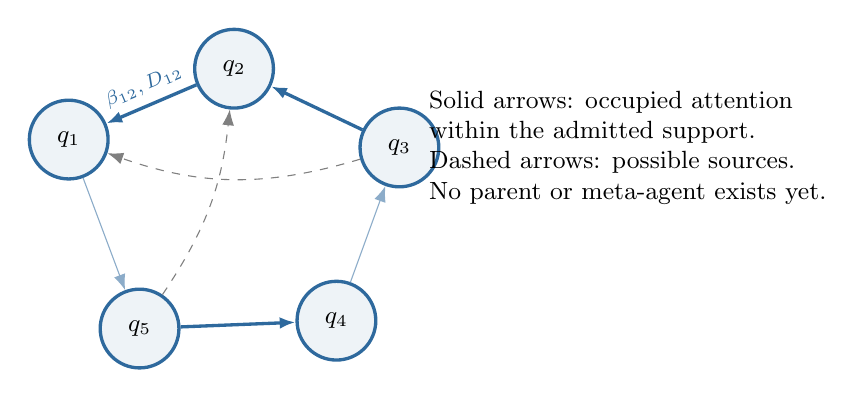
\begin{tikzpicture}[
 agent/.style={circle,draw=agentblue,very thick,fill=agentblue!8,minimum size=10mm,font=\small},
 active/.style={-{Latex[length=2mm]},agentblue,very thick},
 weak/.style={-{Latex[length=2mm]},agentblue!55,thin},
 possible/.style={-{Latex[length=2mm]},gray,dashed}
]
\node[agent] (q1) at (0,1.2) {$q_1$};
\node[agent] (q2) at (2.1,2.1) {$q_2$};
\node[agent] (q3) at (4.2,1.1) {$q_3$};
\node[agent] (q4) at (3.4,-1.1) {$q_4$};
\node[agent] (q5) at (0.9,-1.2) {$q_5$};
\draw[active] (q2) -- node[above,sloped,font=\scriptsize] {$\beta_{12},D_{12}$} (q1);
\draw[active] (q3) -- (q2);
\draw[weak] (q4) -- (q3);
\draw[active] (q5) -- (q4);
\draw[weak] (q1) -- (q5);
\draw[possible] (q3) to[bend left=18] (q1);
\draw[possible] (q5) to[bend right=14] (q2);
\node[align=left,font=\small] at (7.1,1.1) {Solid arrows: occupied attention\\within the admitted support.\\Dashed arrows: possible sources.\\No parent or meta-agent exists yet.};
\end{tikzpicture}
\caption{Stage I is a network of agents only.  The transported divergence sets an edge energy, and the correct row free energy sets the conditional attention.  Coherent subgraphs may appear, but no new probabilistic parent has yet been constructed.}
\label{fig:fine-agent-network}
\end{figure}

\section{The literal negative-chemical-potential correspondence}

At any instant one may define $N_{ij}:=D_{ij}$ and $\mu_{ij}:=-\beta_{ij}$.  Then
\begin{equation}
 \beta_{ij}D_{ij}=-\mu_{ij}N_{ij},
 \label{eq:literal-grand-term}
\end{equation}
and
\begin{equation}
 d(\beta_{ij}D_{ij})
 =D_{ij}d\beta_{ij}+\beta_{ij}dD_{ij}
 =-N_{ij}d\mu_{ij}-\mu_{ij}dN_{ij}.
 \label{eq:literal-differential}
\end{equation}
The algebra remains correct when both quantities evolve.  The limitation is that relative entropy is generally neither an extensive particle number nor a conserved quantity exchanged with a reservoir.  The learned $\beta_{ij}$ is a normalized conditional occupation, not an imposed intensive field.  Equation~\eqref{eq:literal-grand-term} is therefore a generalized Legendre correspondence rather than yet a physical chemical-potential law.

The full row objective also prevents a trivial failure.  If $\beta_{ij}$ were unconstrained in the bare product, then $\partial(\beta_{ij}D_{ij})/\partial\beta_{ij}=D_{ij}\geq0$, and descent would drive every positive coupling toward zero.  The simplex and relative-entropy term instead cause the row to redistribute toward low-energy sources.

\section{Stage II: a grand-canonical network topology}

To make edge number fluctuate, introduce a binary occupation $a_{ij}\in\{0,1\}$ and its mean $\rho_{ij}=\E[a_{ij}]$.  Let $\pi_{ij}^{E}\in(0,1)$ be a reference occupation probability.  A general edge energy can combine belief mismatch, model mismatch, boundary cost, and retention gain:
\begin{equation}
 \epsilon_{ij}
 =J_qD_{ij}^{q}+J_mD_{ij}^{m}+B_{ij}-G_{ij},
 \label{eq:edge-energy}
\end{equation}
where
\begin{equation}
 D_{ij}^{q}=\KL\left(q_i^b\Vert(\Omega_{ij}^b)\push q_j^b\right),
 \qquad
 D_{ij}^{m}=\KL\left(q_i^m\Vert(\Omega_{ij}^m)\push q_j^m\right).
\end{equation}
The costs $B_{ij}$ and gains $G_{ij}$ must be declared; KL geometry does not supply them automatically.

\begin{definition}[Grand-canonical edge functional]
For edge temperature $\tau_E>0$ and chemical potentials $\mu_{ij}$, define
\begin{align}
 \cG[q,\rho]
 &=\cF_{\mathrm{agents}}[q]
 +\sum_{ij}\rho_{ij}\epsilon_{ij}[q]
 -\sum_{ij}\mu_{ij}\rho_{ij}
 \nonumber\\
 &\quad+\tau_E\sum_{ij}
 \KL\left(\Bern(\rho_{ij})\Vert\Bern(\pi_{ij}^{E})\right).
 \label{eq:grand-functional}
\end{align}
The expected edge number is $\langle N_E\rangle=\sum_{ij}\rho_{ij}$.
\end{definition}

\begin{proposition}[Grand-canonical edge occupation]
For fixed beliefs and independent binary edges, Eq.~\eqref{eq:grand-functional} has the unique minimizer
\begin{equation}
 \boxed{
 \rho_{ij}^*
 =\sigmoid\left[
 \logit(\pi_{ij}^{E})
 +\frac{\mu_{ij}-\epsilon_{ij}}{\tau_E}
 \right].}
 \label{eq:fermi-edge-occupation}
\end{equation}
The minimized edge grand potential is
\begin{equation}
 \Phi_E
 =-\tau_E\sum_{ij}\log\left[
 1-\pi_{ij}^{E}
 +\pi_{ij}^{E}\exp\left(\frac{\mu_{ij}-\epsilon_{ij}}{\tau_E}\right)
 \right],
 \label{eq:edge-grand-potential}
\end{equation}
and the exact conjugacy is
\begin{equation}
 -\frac{\partial\Phi_E}{\partial\mu_{ij}}=\rho_{ij}^*.
 \label{eq:chemical-conjugacy}
\end{equation}
\end{proposition}

The chemical potential now couples to an actual fluctuating count.  Positive $\mu_{ij}$ favors an edge and negative $\mu_{ij}$ suppresses it.  In the low-temperature limit the edge is occupied when $\mu_{ij}>\epsilon_{ij}$.  The grand occupation and canonical attention have distinct roles: $\rho_{ij}$ answers whether the edge exists, while $\beta_{ij}$ answers which admitted source is selected conditional on a receiver event.  When $m_i:=\sum_j\rho_{ij}>0$, one may set $\beta_{ij}=\rho_{ij}/m_i$.  The count-bearing intensity is $m_i$, not the normalized row.

\begin{figure}[t]
\centering
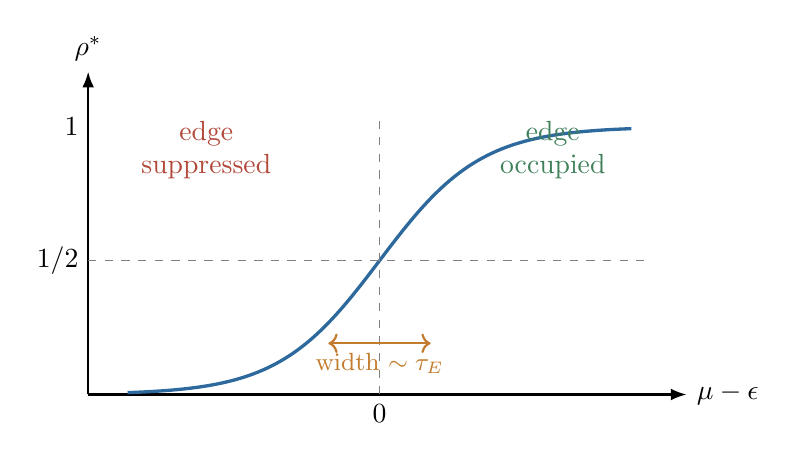
\begin{tikzpicture}[x=1cm,y=1cm]
\draw[-{Latex[length=2mm]},thick] (0,0) -- (7.6,0) node[right] {$\mu-\epsilon$};
\draw[-{Latex[length=2mm]},thick] (0,0) -- (0,4.1) node[above] {$\rho^*$};
\draw[agentblue,very thick,domain=-3.2:3.2,samples=100,smooth]
 plot ({3.7+\x},{3.4/(1+exp(-1.55*\x))});
\draw[gray,dashed] (3.7,0) -- (3.7,3.5);
\draw[gray,dashed] (0,1.7) -- (7.1,1.7);
\node[below] at (3.7,0) {$0$};
\node[left] at (0,1.7) {$1/2$};
\node[left] at (0,3.4) {$1$};
\node[align=center,text=edgered] at (1.5,3.1) {edge\\suppressed};
\node[align=center,text=parentgreen] at (5.9,3.1) {edge\\occupied};
\draw[<->,fieldorange,thick] (3.05,0.65) -- node[below,font=\small] {width $\sim\tau_E$} (4.35,0.65);
\end{tikzpicture}
\caption{Grand-canonical edge occupation.  Chemical potential competes against gauge-covariant mismatch and other edge costs.  The zero-temperature step is rounded over a scale set by $\tau_E$.}
\label{fig:edge-threshold}
\end{figure}

\section{Joint descent of the fine network and topology}

Let the belief laws carry their Fisher--Rao geometry, edge occupations their Bernoulli Fisher geometry, and gauge frames a declared positive mobility.  A joint flow is
\begin{align}
 \dot q_i&=-\Gamma_i^q\grad_{q_i}^{F}\cG,
 \label{eq:q-flow}\\
 \dot\rho_{ij}&=-\Gamma_{ij}^{E}\rho_{ij}(1-\rho_{ij})
 \frac{\partial\cG}{\partial\rho_{ij}},
 \label{eq:rho-flow}\\
 \dot\phi_i&=-\Gamma_i^{\phi}\grad_{\phi_i}\cG.
 \label{eq:gauge-flow}
\end{align}
The factor $\rho(1-\rho)$ is the inverse Bernoulli Fisher information.  Because $D_{ij}$ depends on beliefs and transports, node states, frames, and topology coevolve.

\begin{proposition}[Lyapunov law under fixed controls]
If chemical potentials, temperatures, reference occupations, observation records, and boundary data are fixed, all mobilities are positive, and every update uses the full derivative of the same scalar, then
\begin{align}
 \frac{d\cG}{dt}
 &=-\sum_i\Gamma_i^q\lVert\grad_{q_i}^{F}\cG\rVert_F^2
 -\sum_{ij}\Gamma_{ij}^{E}\rho_{ij}(1-\rho_{ij})
 \left(\frac{\partial\cG}{\partial\rho_{ij}}\right)^2
 \nonumber\\
 &\quad-\sum_i\Gamma_i^{\phi}\lVert\grad_{\phi_i}\cG\rVert^2
 \leq0.
 \label{eq:lyapunov-law}
\end{align}
\end{proposition}

Annealing can yield metastability, symmetry breaking, and slow reorganization, but fixed-control gradient flow still relaxes.  With driven reservoirs,
\begin{equation}
 \frac{d\cG}{dt}
 =-\mathcal D-\sum_{ij}\rho_{ij}\dot\mu_{ij}
 +\frac{\partial\cG}{\partial\tau_E}\dot\tau_E
 +\text{boundary and reference-law work},
 \label{eq:driven-balance}
\end{equation}
where $\mathcal D\geq0$.  Sustained nonequilibrium requires drive, open flux, stochastic forcing, delay, nonreciprocity, or an antisymmetric kinetic sector.

\section{Gauge covariance}

Under a local frame change,
\begin{equation}
 q_i\mapsto(g_i)\push q_i,
 \qquad
 \Omega_{ij}\mapsto g_i\Omega_{ij}g_j^{-1}.
 \label{eq:gauge-action}
\end{equation}
Then $r_{ij}\mapsto(g_i)\push r_{ij}$ and invariance of relative entropy under a common measurable bijection gives
\begin{equation}
 \KL\left((g_i)\push q_i\Vert(g_i)\push r_{ij}\right)
 =\KL(q_i\Vert r_{ij}).
 \label{eq:gauge-kl-invariance}
\end{equation}
If $B_{ij}$, $G_{ij}$, $\mu_{ij}$, $\tau_E$, and $\pi_{ij}^{E}$ are gauge scalars, the edge occupation and grand potential are gauge-invariant.  This conclusion is distribution-general.  Gaussian formulas may evaluate $D_{ij}$ cheaply, but Gaussianity is not part of the theorem.

\section{A mean-field coherence instability}

Let $m$ be a scalar coherence order parameter for a candidate block, with $m=0$ incoherent, and assume
\begin{equation}
 D(m)=D_0-cm^2,
 \qquad c>0.
 \label{eq:mismatch-order-parameter}
\end{equation}
For a representative internal edge, consider
\begin{align}
 \cG_{\mathrm{mf}}(m,\rho)
 &=\frac{a}{2}m^2+\frac{b}{4}m^4
 +\rho J(D_0-cm^2)-\mu\rho
 \nonumber\\
 &\quad+\tau_E\left[\rho\log\rho+(1-\rho)\log(1-\rho)\right],
 \qquad b>0.
 \label{eq:mean-field-grand-potential}
\end{align}
Eliminating $\rho$ gives
\begin{equation}
 \rho^*(m)=\sigmoid\left(\frac{\mu-JD_0+Jcm^2}{\tau_E}\right)
 \label{eq:mean-field-occupation}
\end{equation}
and
\begin{equation}
 \cG_{\mathrm{red}}(m)
 =\frac{a}{2}m^2+\frac{b}{4}m^4
 -\tau_E\log\left[1+\exp\left(\frac{\mu-JD_0+Jcm^2}{\tau_E}\right)\right].
 \label{eq:mean-field-reduced}
\end{equation}
Writing $\rho_0=\sigmoid((\mu-JD_0)/\tau_E)$, the quadratic coefficient is $(a-2Jc\rho_0)/2$.  The incoherent state loses local stability when
\begin{equation}
 \boxed{2Jc\rho_0>a.}
 \label{eq:coherence-instability}
\end{equation}
The quartic coefficient receives the correction
\begin{equation}
 -\frac{J^2c^2}{2\tau_E}\rho_0(1-\rho_0).
 \label{eq:quartic-correction}
\end{equation}
A positive final quartic coefficient predicts a continuous mean-field transition.  A negative coefficient requires higher-order stabilization and permits a discontinuous transition with hysteresis.  This is a conditional reduction, not a theorem about the full network.

The occupation susceptibility is
\begin{equation}
 \frac{\partial\rho_0}{\partial\mu}
 =\frac{\rho_0(1-\rho_0)}{\tau_E},
 \label{eq:edge-susceptibility}
\end{equation}
which peaks near half occupation.  This gives a direct experimental diagnostic.

\section{Stage III: formation of a pointwise meta-agent}

Let $n_{iA}\in\{0,1\}$ indicate membership of fine agent $i$ in candidate parent $A$, with $\rho_{iA}=\E[n_{iA}]$.  Define
\begin{equation}
 \epsilon_{iA}
 =J_q\KL\left(q_i^b\Vert(\Omega_{iA}^b)\push q_A^b\right)
 +J_m\KL\left(q_i^m\Vert(\Omega_{iA}^m)\push q_A^m\right)
 +B_{iA}-G_{iA}.
 \label{eq:membership-energy}
\end{equation}
The membership grand potential is
\begin{align}
 \cG_A^{\mathrm{mem}}
 &=\sum_i\rho_{iA}\epsilon_{iA}
 -\mu_A\sum_i\rho_{iA}
 \nonumber\\
 &\quad+\tau_A\sum_i
 \KL\left(\Bern(\rho_{iA})\Vert\Bern(\pi_{iA})\right),
 \label{eq:membership-grand-potential}
\end{align}
so
\begin{equation}
 \rho_{iA}^*
 =\sigmoid\left[
 \logit(\pi_{iA})+\frac{\mu_A-\epsilon_{iA}}{\tau_A}
 \right].
 \label{eq:membership-probability}
\end{equation}
The expected parent size is $\langle N_A\rangle=\sum_i\rho_{iA}$ and is conjugate to $\mu_A$.

Membership does not itself construct a parent law.  Let $I_A$ be the fine variables selected for a candidate parent and let $C_A$ be a normalized coarse Markov channel fixed independently of the current recognition law and admitted observation.  At one fixed structural configuration and base point, the full parent datum is
\begin{equation}
 \boxed{
 \mathbb Q_A=(C_A)\push\mathbb Q_{I_A},
 \qquad
 \mathbb P_A=(\operatorname{id}_{O}\times C_A)\push\mathbb P_{I_A},
 \qquad
 \boldsymbol\Pi_A=(C_A)\push\boldsymbol\Pi_{I_A}.}
 \label{eq:parent-full-laws}
\end{equation}
The parent belief and model laws must be projections or disintegrations of these full laws.  An evaluator must map a parent model presentation to a normalized generative kernel on the retained interface.  Only then does the coherent block define a pointwise probabilistic meta-agent datum.

The two constructions solve different problems.  Equation~\eqref{eq:membership-grand-potential} explains why a fine agent is statistically favored as a member.  Equation~\eqref{eq:parent-full-laws} defines what probabilistic object the parent carries.  Membership without a coarse channel gives a cluster but no parent.  A coarse channel for a declared block gives a parent but does not explain why that block formed.

Independent Bernoulli memberships permit overlapping parents.  A categorical constraint $\sum_A\rho_{iA}=1$ instead gives canonical exclusive assignment.  A unique hierarchy or latent directed acyclic graph does not follow without further exclusion, geometry, or model-selection terms.

\begin{figure}[t]
\centering
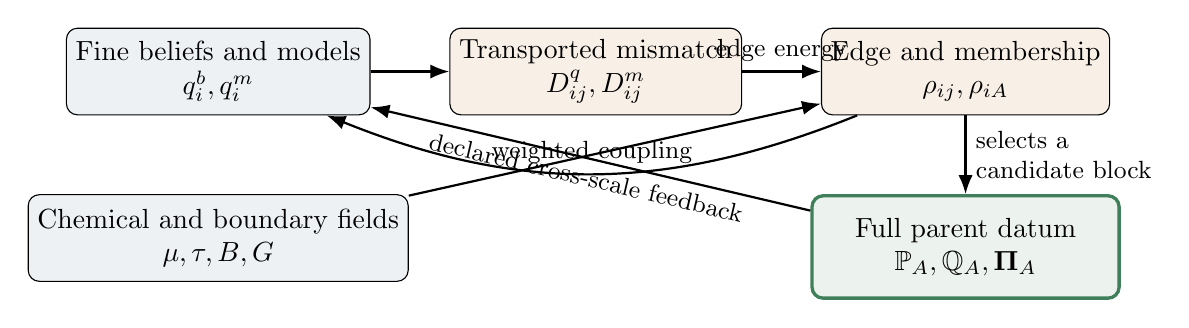
\begin{tikzpicture}[
 box/.style={draw,rounded corners,align=center,minimum width=31mm,minimum height=11mm,fill=softgray},
 ebox/.style={draw,rounded corners,align=center,minimum width=34mm,minimum height=11mm,fill=fieldorange!12},
 pbox/.style={draw=parentgreen,very thick,rounded corners,align=center,minimum width=39mm,minimum height=13mm,fill=parentgreen!10},
 arr/.style={-{Latex[length=2.4mm]},thick}
]
\node[box] (beliefs) {Fine beliefs and models\\$q_i^b,q_i^m$};
\node[ebox,right=of beliefs] (mismatch) {Transported mismatch\\$D_{ij}^q,D_{ij}^m$};
\node[ebox,right=of mismatch] (occupancy) {Edge and membership\\$\rho_{ij},\rho_{iA}$};
\node[pbox,below=of occupancy] (parent) {Full parent datum\\$\mathbb P_A,\mathbb Q_A,\boldsymbol\Pi_A$};
\node[box,below=of beliefs] (field) {Chemical and boundary fields\\$\mu,\tau,B,G$};
\draw[arr] (beliefs) -- (mismatch);
\draw[arr] (mismatch) -- node[above,font=\small] {edge energy} (occupancy);
\draw[arr] (field) -- (occupancy);
\draw[arr] (occupancy) -- node[right,font=\small,align=left] {selects a\\candidate block} (parent);
\draw[arr] (parent) -- node[below,sloped,font=\small] {declared cross-scale feedback} (beliefs);
\draw[arr] (occupancy) to[bend left=22] node[above,font=\small] {weighted coupling} (beliefs);
\end{tikzpicture}
\caption{Stage III separates formation from construction.  Grand occupations select a candidate membership, while a coarse channel constructs the full parent probability laws.  The feedback arrow is an additional dynamical coupling, not a consequence of membership alone.}
\label{fig:formation-loop}
\end{figure}

\section{Stage IV: a network of meta-agents and recursive scale formation}

Once several parent data have been constructed, the parents can become nodes of a new network.  Let $\ell$ label scale and $A,B$ label agents or meta-agents at that scale.  Their transported mismatch is
\begin{equation}
 D_{AB}^{(\ell)}
 =\KL\left(q_A^{(\ell)}\middle\Vert
 (\Omega_{AB}^{(\ell)})\push q_B^{(\ell)}\right).
 \label{eq:scale-divergence}
\end{equation}
Each scale can carry canonical source rows $\beta_{AB}^{(\ell)}$ and grand occupations $\rho_{AB}^{(\ell)}$.  Its network functional has the recursive form
\begin{align}
 \cG^{(\ell)}
 &=\cF_{\mathrm{agents}}^{(\ell)}
 +\sum_{A,B}\rho_{AB}^{(\ell)}\epsilon_{AB}^{(\ell)}
 -\sum_{A,B}\mu_{AB}^{(\ell)}\rho_{AB}^{(\ell)}
 \nonumber\\
 &\quad+\tau_E^{(\ell)}\sum_{A,B}
 \KL\left(\Bern(\rho_{AB}^{(\ell)})
 \Vert\Bern(\pi_{AB}^{E,(\ell)})\right).
 \label{eq:scale-grand-potential}
\end{align}
This expression is legitimate only after the parent laws and transports have been constructed.  Replacing fine indices by block indices does not prove RG closure.

A tower can be organized as
\begin{equation}
 \cG_{\mathrm{tower}}
 =\sum_{\ell=0}^{L}\lambda_{\ell}\cG^{(\ell)}
 +\sum_{\ell=0}^{L-1}\cC^{(\ell,\ell+1)},
 \label{eq:tower-grand-potential}
\end{equation}
where $\cC^{(\ell,\ell+1)}$ contains coarse-channel compatibility, retained-boundary, conditional-information-loss, and reconstruction-defect terms.  These terms prevent double counting when parent and child descriptions refer to the same evidence or interaction record.

Scale-dependent chemical potentials control expected populations across levels.  They can favor many small parents, a few large parents, or overlapping organizations.  VFE alone does not fix them; they require a boundary condition, hyperprior, conservation rule, or a higher-scale variational sector.  Pointwise construction also does not give a geometric meta-agent over an overlap region.  Local sections, transition maps, cocycles, and regular handling of membership or stabilizer changes remain separate obligations.

\begin{figure}[t]
\centering
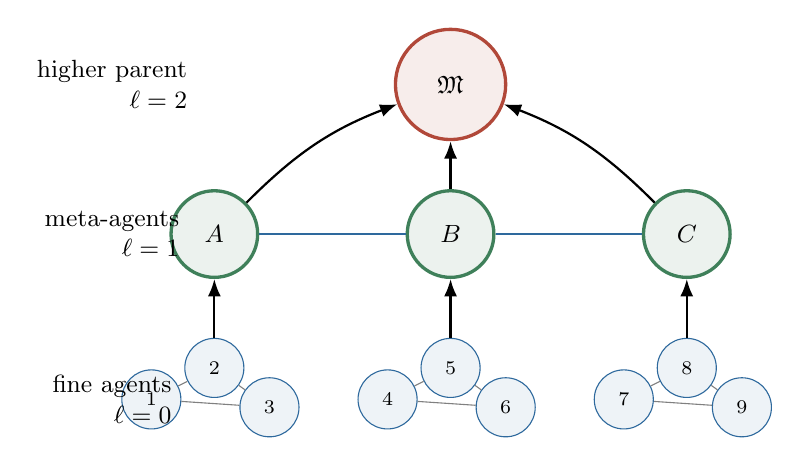
\begin{tikzpicture}[
 fine/.style={circle,draw=agentblue,fill=agentblue!8,minimum size=7.5mm,font=\scriptsize},
 meta/.style={circle,draw=parentgreen,very thick,fill=parentgreen!10,minimum size=11mm,font=\small},
 super/.style={circle,draw=edgered,very thick,fill=edgered!10,minimum size=14mm,font=\small},
 up/.style={-{Latex[length=2.2mm]},thick},
 net/.style={gray,thin}
]
\node[fine] (a1) at (0,0) {$1$}; \node[fine] (a2) at (0.8,0.4) {$2$}; \node[fine] (a3) at (1.5,-0.1) {$3$};
\node[fine] (a4) at (3,0) {$4$}; \node[fine] (a5) at (3.8,0.4) {$5$}; \node[fine] (a6) at (4.5,-0.1) {$6$};
\node[fine] (a7) at (6,0) {$7$}; \node[fine] (a8) at (6.8,0.4) {$8$}; \node[fine] (a9) at (7.5,-0.1) {$9$};
\draw[net] (a1)--(a2)--(a3)--(a1); \draw[net] (a4)--(a5)--(a6)--(a4); \draw[net] (a7)--(a8)--(a9)--(a7);
\node[meta] (A) at (0.8,2.1) {$A$}; \node[meta] (B) at (3.8,2.1) {$B$}; \node[meta] (C) at (6.8,2.1) {$C$};
\draw[up] (a2)--(A); \draw[up] (a5)--(B); \draw[up] (a8)--(C);
\draw[agentblue,thick] (A)--(B)--(C);
\node[super] (M) at (3.8,4.0) {$\mathfrak M$};
\draw[up] (B)--(M); \draw[up] (A) to[bend left=12] (M); \draw[up] (C) to[bend right=12] (M);
\node[align=right,font=\small] at (-0.5,0) {fine agents\\$\ell=0$};
\node[align=right,font=\small] at (-0.5,2.1) {meta-agents\\$\ell=1$};
\node[align=right,font=\small] at (-0.5,4.0) {higher parent\\$\ell=2$};
\end{tikzpicture}
\caption{Stage IV iterates only after each parent has a full probability law and retained interface.  The vertical arrows denote declared coarse channels, not mere averaging.  Horizontal links at each level have their own canonical rows and possible grand occupations.}
\label{fig:recursive-hierarchy}
\end{figure}

\section{Stage V: emergent agency and participatory nonequilibrium}

No primitive action or plan variable is needed to form coherent higher-scale organization.  Fine beliefs, generative-model laws, edge occupations, and parent memberships can evolve under one variational functional.  What emerges first is a persistent probabilistic organization or meta-agent datum, not automatically an autonomous agent.

A participatory extension lets a coarse parent modify fine-scale chemical fields or edge energies, for example
\begin{equation}
 \mu_{ij}=\mu_{ij}^{(0)}+\lambda M_A(\mathbb Q_A,\boldsymbol\Pi_A).
 \label{eq:participatory-field}
\end{equation}
This closes a cross-scale feedback loop: fine agents support the parent, while the parent changes which fine interactions are favorable.  If every variable remains in one reciprocal time-independent scalar and follows its gradient, the enlarged system still obeys a Lyapunov law.  Feedback can create multistability and long transients, but it does not by itself sustain nonequilibrium.

Sustained nonequilibrium requires open boundary flux, a time-dependent reservoir, stochastic drive, delay, nonreciprocal coupling, or an antisymmetric kinetic sector.  A Wheelerian interpretation becomes mathematically substantive only when it declares which parent variables modify which fine kernels, accounts for the corresponding work or flux, and identifies an observable distinguishing the participatory model from an ordinary hierarchical latent-variable model.

\section{Predictions and falsification program}

Sweeping $\mu$ at fixed $\tau_E$ should change mean degree and expected parent size according to the logistic occupation law.  The response should peak near half occupation.  Coupled belief--edge descent should produce a feedback between decreasing transported KL and increasing occupation.  If Eq.~\eqref{eq:coherence-instability} is crossed, the incoherent mean-field state should lose stability.  Hysteresis would indicate that the effective quartic term has changed sign and higher-order stabilization matters.  Finite-size scaling of susceptibility, largest-parent fraction, correlation length, and residence times is required before calling the reorganization a phase transition in the strict statistical-mechanical sense.

The proposed model fails in its own domain if the implemented scalar differs from Eq.~\eqref{eq:grand-functional}, if the frozen-belief edge update fails Eq.~\eqref{eq:fermi-edge-occupation}, if gauge changes alter occupation probabilities, or if a claimed full-gradient implementation increases $\cG$ under fixed controls and positive mobilities.  The physical interpretation remains unproved even if every mathematical test passes unless a physical energy scale, reservoir, and entropy-production accounting are independently identified.

\section{Conclusion}

The coevolution of $\beta_{ij}$ and $D_{ij}$ turns the fine-agent system into an annealed Gibbs network.  The exact row free energy is the energy-plus-relative-entropy expression in Eq.~\eqref{eq:row-free-energy}; omitting its entropy term changes the model.  The identity $\beta_{ij}D_{ij}=-\mu_{ij}N_{ij}$ is a valid generalized Legendre analogy, but a normalized attention row is more naturally an occupation probability than a chemical potential.

A clean grand-canonical extension introduces separate fluctuating edge and membership variables.  Transported KL becomes gauge-invariant bond frustration, and chemical potential controls the number of relationships or members.  This yields an ordered construction: first an adaptive network of agents, then variable topology, then pointwise meta-agent formation, then networks of meta-agents across scales, and finally a participatory nonequilibrium extension.  Each stage adds a typed object and a new falsifier.  The construction supplies a concrete route from variational evolution to higher-scale organization, but autonomous agency, global geometric gluing, unique hierarchy, physical thermodynamics, and sustained nonequilibrium remain distinct open problems.

\begin{thebibliography}{9}

\bibitem{Friston2010}
K. Friston,
``The free-energy principle: a unified brain theory?,''
\emph{Nature Reviews Neuroscience}, vol. 11, pp. 127--138, 2010.
\href{https://doi.org/10.1038/nrn2787}{doi:10.1038/nrn2787}.

\bibitem{Jaynes1957}
E. T. Jaynes,
``Information theory and statistical mechanics,''
\emph{Physical Review}, vol. 106, pp. 620--630, 1957.
\href{https://doi.org/10.1103/PhysRev.106.620}{doi:10.1103/PhysRev.106.620}.

\bibitem{ParkNewman2004}
J. Park and M. E. J. Newman,
``Statistical mechanics of networks,''
\emph{Physical Review E}, vol. 70, 066117, 2004.
\href{https://doi.org/10.1103/PhysRevE.70.066117}{doi:10.1103/PhysRevE.70.066117}.

\bibitem{GrossBlasius2008}
T. Gross and B. Blasius,
``Adaptive coevolutionary networks: a review,''
\emph{Journal of the Royal Society Interface}, vol. 5, pp. 259--271, 2008.
\href{https://doi.org/10.1098/rsif.2007.1229}{doi:10.1098/rsif.2007.1229}.

\end{thebibliography}

\end{document}
